\section{Contexto y estado del arte}
\label{sec:ctx_estart}

En los últimos años, la predicción del tráfico se ha convertido en un campo de investigación clave dentro de los \acrlong{its}, impulsado por la disponibilidad creciente de datos en tiempo real y los avances en el aprendizaje automático. El objetivo principal es anticipar las condiciones del tráfico con suficiente precisión como para facilitar la toma de decisiones, tanto por parte de los operadores como de los usuarios de la red vial.

La problemática de la predicción del tráfico en entornos urbanos y regionales como Bizkaia presenta una elevada complejidad, debido a la naturaleza altamente dinámica y no lineal del flujo vehicular, así como por la influencia de factores exógenos como el clima, los eventos especiales o los accidentes. Esta complejidad ha motivado el desarrollo de una gran variedad de enfoques, desde modelos estadísticos clásicos hasta sofisticadas arquitecturas de aprendizaje profundo.

Este capítulo tiene como objetivo ofrecer un panorama de las principales técnicas, modelos y tecnologías utilizadas en la predicción del tráfico. A partir de una revisión sistemática de la literatura científica más relevante, se presentarán los enfoques predominantes y se analizará su aplicabilidad al caso concreto de Bizkaia. Finalmente, se establecerá un marco comparativo que servirá como punto de partida para justificar la solución propuesta en este trabajo.

\subsection{Técnicas existentes para la predicción del tráfico}

En la literatura se han desarrollado diversas técnicas para la predicción del tráfico, desde modelos estadísticos clásicos hasta enfoques basados en aprendizaje profundo. Entre las principales categorías se encuentran:

\begin{itemize}
	\item \textbf{Modelos estadísticos lineales}: como \acrlong{arima}, Kalman Filter o regresiones lineales, empleados tradicionalmente en la predicción de series temporales de tráfico \cite{forecastSarima, forecastArimaLtsm, forecastKalman, liu2020congestion}.
	\item \textbf{Modelos basados en Support Vector Regression}: \acrlong{svr}, \acrlong{rf}, \acrlong{knn}, que han mostrado eficacia en contextos con datos limitados y estructuras menos complejas \cite{omar2024, forecastRf, forecastKnn}.
	\item \textbf{Redes neuronales profundas}:
	\begin{itemize}
		\item \acrlong{rnn}, y variantes como \acrlong{lstm} y \acrlong{gru}, diseñadas para capturar dependencias temporales a corto y largo plazo en series de tráfico \cite{hochreiter1997long, cho2014gru, zhao2017lstm, ma2022cnn_gru}.
		\item \acrlong{gnn}, incluyendo \acrlong{gcn} y \acrlong{gat} (adaptadas a redes viarias), que permiten modelar explícitamente la topología de la red viaria y las relaciones entre distintos nodos \cite{forecastGgnn, forecastGnn}.
		\item Modelos basados en transformer, que han demostrado una capacidad sobresaliente para captar dependencias espaciotemporales y superar limitaciones de modelos anteriores \cite{trafficformer}.
	\end{itemize}
\end{itemize}

En las siguientes secciones, se revisarán con más detalle los fundamentos y aplicaciones de estas técnicas, poniendo el foco en los trabajos más relevantes que hayan utilizado estos enfoques en entornos comparables al del presente proyecto.

\subsubsection*{Modelos estadísticos tradicionales}

Los modelos estadísticos tradicionales han sido fundamentales en la predicción del tráfico, especialmente en contextos donde se dispone de datos históricos limitados o se requiere una interpretación sencilla de los resultados. Estos modelos, incluyendo ARIMA, filtros de Kalman y regresiones lineales, permiten capturar patrones temporales y tendencias en los datos de tráfico, ofreciendo una base sólida para el desarrollo de sistemas de transporte inteligentes.

Los modelos \acrlong{arima} son herramientas estadísticas utilizadas para analizar y predecir series temporales. En el ámbito del tráfico, han demostrado ser eficaces para prever flujos vehiculares a corto plazo, especialmente en situaciones con patrones estacionales o tendencias lineales.

Por ejemplo, \cite{forecastArimaLtsm} aplicaron modelos \acrshort{arima} y \acrshort{lstm} para predecir el flujo de tráfico en la intersección de Muhima, Kigali, concluyendo que la combinación de ambos modelos mejora la precisión de las predicciones.

Asimismo, \cite{forecastSarima} propusieron un esquema de predicción utilizando el modelo \acrlong{sarima} para prever el flujo de tráfico a corto plazo con datos limitados, demostrando que es posible obtener predicciones precisas utilizando solo tres días de datos históricos.

El filtro de Kalman es un algoritmo recursivo que estima el estado de un sistema dinámico a partir de una serie de mediciones observadas, que contienen ruido y otras inexactitudes. En la predicción del tráfico, se utiliza para estimar y prever el flujo vehicular en tiempo real, adaptándose a cambios abruptos y condiciones variables.​

\cite{forecastKalman} emplearon el filtro de Kalman para predecir el flujo de tráfico a corto plazo en una carretera urbana de Dhaka, Bangladesh. El modelo logró un \acrlong{mape} del 14.62\%, indicando una precisión aceptable para aplicaciones prácticas.

La regresión lineal es una técnica estadística que modela la relación entre una variable dependiente y una o más variables independientes. En el contexto del tráfico, se ha utilizado para prever velocidades y flujos vehiculares basándose en variables como el tiempo, la densidad y la ocupación de la vía.​

Por ejemplo, \cite{liu2020congestion} desarrollaron un modelo de predicción del tiempo de congestión del tráfico utilizando análisis de regresión múltiple y análisis de supervivencia. El estudio demostró que el modelo de regresión lineal múltiple puede predecir con precisión el tiempo de congestión del tráfico, con un grado de ajuste entre el valor predicho y el valor real superior a 0.96. Este enfoque permitió identificar las características de distribución y duración de la congestión, proporcionando una base sólida para la predicción del tráfico en entornos urbanos.​

Sin embargo, estudios recientes han señalado limitaciones en la regresión lineal para capturar relaciones no lineales complejas en los datos de tráfico. Por ejemplo, en un análisis exhaustivo, se comparó el rendimiento de la regresión lineal con modelos más avanzados como \acrlong{rf} y XGBoost, encontrando que la regresión lineal presenta un ajuste deficiente y errores significativos en la predicción de velocidades de tráfico.

\subsubsection*{Modelos clásicos de Machine Learning}

Los modelos clásicos de machine learning son métodos estadísticos avanzados capaces de abordar problemas complejos y no lineales. A continuación se describen brevemente tres técnicas destacadas: \acrlong{svr}, \acrlong{rf} y \acrlong{knn}, incluyendo ejemplos recientes de aplicaciones en la predicción del tráfico.

En cuanto a \acrfull{svr}, es una técnica basada en \acrfull{svm} que utiliza una función kernel para transformar el espacio de entrada original a uno de mayor dimensión, permitiendo modelar relaciones no lineales. El objetivo del \acrshort{svr} es identificar una función que tenga, como máximo, un error preestablecido (denominado \textit{margen}) respecto a los datos reales.

En el contexto de predicción de tráfico, \acrshort{svr} se ha mostrado eficaz debido a su robustez ante ruido y capacidad de generalización con muestras pequeñas. Por ejemplo, un estudio reciente aplicó \acrshort{svr} para predecir el volumen de tráfico a corto plazo utilizando datos de flujo vehicular recolectados en áreas urbanas, mostrando una precisión significativa en comparación con métodos \acrshort{lstm} de \cite{omar2024}.

\acrfull{rf} es un algoritmo basado en árboles de decisión, que genera múltiples árboles de forma independiente, utilizando subconjuntos aleatorios de datos de entrenamiento (bagging) y variables aleatorias. La predicción final se obtiene por consenso, promediando las predicciones individuales de cada árbol, lo que reduce considerablemente el riesgo de sobreajuste.

En el ámbito del tráfico, \acrshort{rf} es capaz de manejar grandes volúmenes de datos y capturar relaciones no lineales y complejas. Un ejemplo de aplicación es el estudio realizado por \cite{forecastRf}. El estudio tiene como objetivo predecir el flujo de tráfico a corto plazo, considerando patrones espaciales y temporales. Tras el preprocesamiento de datos con el Transformador Cuantil y la exploración de la correlación del flujo de tráfico, se identificaron los hiperparámetros óptimos del modelo mediante la búsqueda de cuadrícula de validación cruzada. El modelo \acrshort{rf} demostró el mejor rendimiento, alcanzando una alta precisión en la predicción del flujo de tráfico.

\acrfull{knn} es uno de los algoritmos más sencillos dentro de los métodos de aprendizaje supervisado. Este método predice el valor de una observación nueva en función de los valores de las K observaciones más cercanas del conjunto de entrenamiento. La cercanía se determina generalmente mediante una métrica de distancia, siendo la distancia euclidiana la más comúnmente utilizada.

A pesar de su simplicidad, \acrshort{knn} es muy eficaz en la predicción de tráfico cuando los patrones de flujo muestran alta dependencia espacial y temporal. Recientemente, \cite{forecastKnn} emplearon \acrshort{knn} para la predicción del tráfico en Bandung, Indonesia, empleando este método e integrado con la aplicación de simulación de movilidad urbana SUMO. El estudio buscó mitigar la congestión de tráfico anual en la ciudad, particularmente en periodos vacacionales. Utilizaron datos históricos de tráfico de Jl. Riau Bandung para predecir el nivel de congestión. La evaluación del rendimiento del método, usando una división de datos para entrenamiento y prueba, demostró una precisión muy alta con diferentes valores de 'k' vecinos considerados.

\subsubsection*{Aprendizaje profundo}

El \textit{Deep Learning} o aprendizaje profundo es un área de \textit{Machine Learning} que utiliza redes neuronales artificiales de múltiples capas para modelar patrones complejos en los datos. Tras varias décadas de relativo estancamiento debido a las limitaciones computacionales y a las críticas vertidas por Minsky y Papert en los años 60 en el libro \textit{Perceptrons: An Introduction to Computational Geometry} \cite{minsky1969perceptrons}, las redes neuronales experimentaron un resurgimiento a partir de la década de los 2000, impulsado por el incremento exponencial de la capacidad de cómputo, la disponibilidad de grandes volúmenes de datos y el avance en algoritmos de entrenamiento. Este renacimiento del interés en las redes profundas se consolidó con el trabajo de \cite{hinton2006reducing}, donde se introdujo una técnica de preentrenamiento capa por capa utilizando autoencoders y máquinas de Boltzmann restringidas para facilitar el entrenamiento de redes neuronales profundas.

Sin embargo, fue en 2012 cuando el aprendizaje profundo irrumpió definitivamente en la comunidad científica, con la publicación de AlexNet, una red convolucional profunda que ganó con gran margen la competición ImageNet Large Scale Visual Recognition Challenge (ILSVRC). En este trabajo, Krizhevsky, Sutskever y Hinton demostraron que las redes profundas entrenadas con \acrlong{gpu} podían superar ampliamente los métodos tradicionales en tareas de visión por computador \cite{krizhevsky2012imagenet}. Este hito marcó el inicio de una nueva era para el aprendizaje profundo, consolidándolo como una de las herramientas más poderosas dentro del campo de la inteligencia artificial.

Actualmente, el aprendizaje profundo se caracteriza por la capacidad de representar funciones no lineales muy complejas gracias a estructuras como las redes neuronales profundas de tipo \acrlong{mlp}. Estas redes constan de múltiples capas ocultas, donde cada capa procesa información progresivamente más abstracta y permite descubrir patrones intrínsecos en grandes volúmenes de datos.

\subsubsection*{Redes neuronales recurrentes}

Las redes neuronales recurrentes (\acrfull{rnn}) han demostrado gran eficacia en la predicción de series temporales en el ámbito del tráfico, gracias a su capacidad para modelar dependencias a largo plazo mediante estructuras como las \acrshort{lstm} \cite{hochreiter1997long} y las \acrshort{gru} \cite{cho2014gru}. Diversos estudios han validado su aplicabilidad en este campo, destacando resultados como los obtenidos por Zhao et al. con \acrshort{lstm}, logrando un error relativo medio (\acrshort{mre}) del 6,41\% en predicción de flujo de tráfico a corto plazo \cite{zhao2017lstm}, o la propuesta de Ma et al., que combinan \acrshort{cnn} y \acrshort{gru} para alcanzar un \acrshort{mape} del 8,60\% en predicción de velocidad \cite{ma2022cnn_gru}. Estas evidencias posicionan a las \acrshort{rnn} y sus variantes como alternativas robustas frente a métodos tradicionales, especialmente en tareas de predicción a corto plazo.

\subsubsection*{Graph Neural Networks}

Las \acrlong{gnn} han permitido extender el aprendizaje profundo a datos no euclidianos como los grafos, resultando especialmente adecuadas para modelar redes de carreteras en sistemas inteligentes de transporte \cite{theoryGnn}. Estas arquitecturas, como las Graph Convolutional Networks (\acrshort{gcn}), introducidas en \cite{theoryGcn}, Graph Attention Networks (\acrshort{gat}), introducidas en \cite{theoryGan} y las Gated Graph Neural Networks (\acrshort{ggnn}), destacan por su capacidad para capturar dependencias espaciales y temporales entre nodos e incorporar mecanismos avanzados como la atención o puertas de control. Diversos estudios han demostrado su efectividad en la predicción del flujo y la densidad del tráfico; por ejemplo, el trabajo de \cite{forecastGgnn} evidencia que las \acrshort{ggnn} superan a otras arquitecturas en precisión, mientras que propuestas como TrafficStream \cite{forecastGnn} combinan \acrshort{gnn} con aprendizaje continuo para adaptarse a cambios dinámicos en los patrones de tráfico.

\subsubsection*{Redes Neuronales con Transformers}

El avance hacia modelos más potentes y versátiles dentro del aprendizaje profundo encontró un punto de inflexión crucial en 2017 con la publicación del influyente artículo \textit{Attention is all you need} por \cite{attentionIsAllYouNeed}. Esta publicación revolucionó el campo del aprendizaje automático al introducir la arquitectura Transformer, una propuesta que eliminaba por completo el uso de estructuras recurrentes como \acrshort{rnn} o \acrshort{lstm}, en favor de un novedoso mecanismo de atención que permitía modelar relaciones de largo alcance en las secuencias de entrada, mediante el cómputo paralelo.

La clave de los Transformers reside en el \textbf{multi-head self-attention}, que otorga al modelo la capacidad de ponderar dinámicamente la importancia relativa de distintos elementos dentro de una secuencia. Este mecanismo, además de ofrecer un rendimiento computacional más eficiente, mejora la capacidad de aprendizaje del modelo frente a secuencias largas o ruidosas, lo que resulta particularmente útil en dominios complejos como la predicción del flujo del tráfico urbano.

A diferencia de las \acrshort{rnn}, que deben procesar las secuencias de manera secuencial, los Transformers permiten el aprendizaje paralelo y la captura simultánea de dependencias tanto locales como globales, lo que ha demostrado ser especialmente relevante para modelar patrones espacio-temporales complejos.

\vspace{0.5cm}

El uso de modelos Transformer en el ámbito de los sistemas inteligentes de transporte ha crecido significativamente en los últimos años, debido a su capacidad para capturar interacciones complejas entre nodos de una red vial y su evolución en el tiempo.

Un estudio reciente y particularmente relevante para este trabajo es el desarrollado por \cite{trafficformer}, titulado \textit{Transformer-based short-term traffic forecasting model considering traffic spatiotemporal correlation}. En este artículo, los autores presentan \textbf{Trafficformer}, un modelo Transformer adaptado específicamente a la predicción del tráfico a corto plazo, integrando correlaciones espacio-temporales mediante máscaras espaciales y representaciones topológicas de la red viaria.

\begin{figure}[H]
	\centering
	\caption{Arquitectura general del modelo Trafficformer \cite{trafficformer}}
	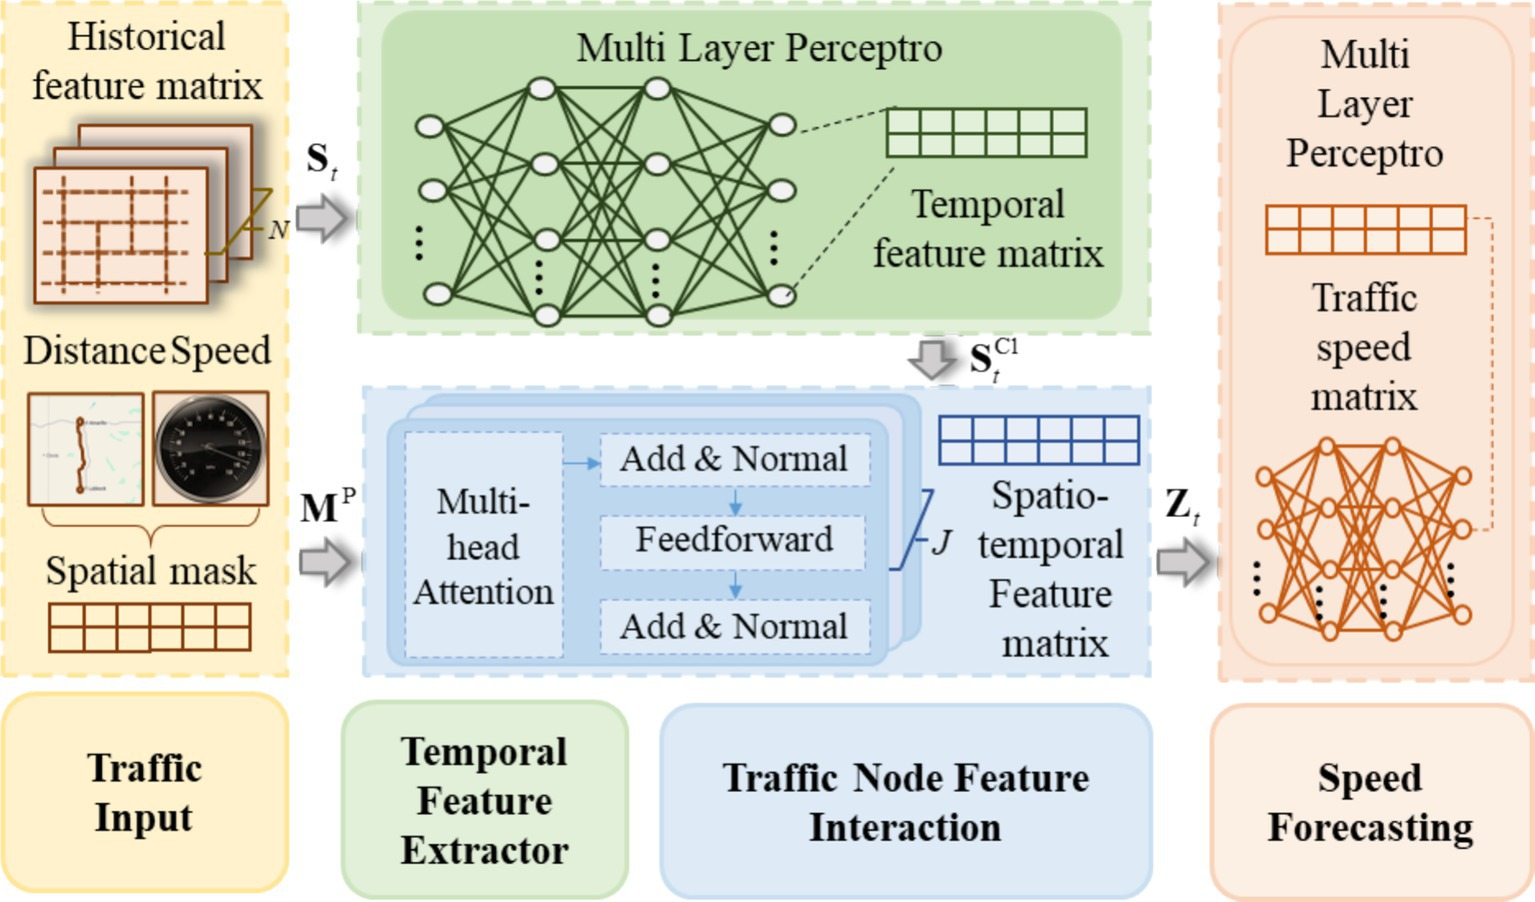
\includegraphics[width=0.9\textwidth]{includes/fnbot-19-1527908-g001.jpg}
	\label{fig:trafficformer}
\end{figure}
\fuente{\citet{trafficformer}}

En cuanto a la arquitectura, el modelo Trafficformer (véase Figura~\ref{fig:trafficformer}) consta de tres módulos fundamentales:
\begin{itemize}
	\item[(1)] Extracción de características temporales mediante \acrlong{mlp}. 
	\item[(2)] Interacción espacial basada en codificadores Transformer con máscaras de atención topológicas. 
	\item[(3)] Predicción de velocidades mediante una red \acrshort{mlp} final. 
\end{itemize}

Esta arquitectura fue evaluada con el conjunto de datos del \textit{Seattle Loop Detector Dataset}, superando a modelos clásicos como ARIMA, \acrshort{svr} y también a redes profundas como \acrshort{lstm}+\acrshort{mlp} y TGG-LSTM, tanto en precisión (\acrshort{mae}, \acrshort{mape}, \acrshort{rmse}) como en eficiencia computacional.

La inclusión de una máscara espacial, que filtra interacciones irrelevantes basándose en la topología vial y el tiempo de viaje entre nodos, permitió al modelo enfocarse en relaciones espacialmente significativas, lo que se tradujo en una mejora del 18\% en precisión frente a modelos equivalentes sin esta optimización. Esta capacidad de interpretar relaciones espaciales relevantes es fundamental en contextos como el tráfico urbano, donde las dependencias no son uniformes ni euclidianas, y dependen del trazado real de la red viaria.

\vspace{0.5cm}

El trabajo de \cite{trafficformer} demuestra que los modelos basados en transformers no sólo son competitivos, sino que se posicionan como una opción de referencia para tareas de predicción del tráfico, permitiendo una mejor generalización, mayor interpretabilidad y adaptabilidad frente a cambios dinámicos en la red.

Este enfoque supone un salto cualitativo respecto a técnicas previas como \acrshort{lstm}, \acrshort{gru} o incluso \acrshort{gnn}, al combinar lo mejor de los modelos de secuencia (captura temporal) con mecanismos estructurados de atención espacial. Además, su arquitectura modular y altamente paralelizable lo convierte en un candidato ideal para despliegues en entornos cloud, edge o híbridos, como los requeridos en la infraestructura del proyecto que nos ocupa.

Por todo ello, este modelo ha sido seleccionado como piedra angular sobre la cual se desarrollará la propuesta metodológica del presente trabajo, tanto en la fase de experimentación como en el diseño arquitectónico del modelo final.

\subsection{Ventajas del uso de Transformers frente a otras arquitecturas}

La arquitectura Transformer representa un avance significativo respecto a los modelos secuenciales (\acrshort{lstm} o \acrshort{gru}) y estructurales (como las \acrshort{gnn}), tanto desde el punto de vista teórico como práctico.

En primer lugar, los modelos secuenciales dependen fuertemente del procesamiento secuencial, lo que limita la paralelización durante el entrenamiento y puede llevar a problemas de desvanecimiento o explosión del gradiente (leer en \cite{desvGradiente}) en secuencias largas. Aunque han demostrado buen rendimiento en predicción temporal, su capacidad para modelar relaciones espaciales complejas es limitada. Por otro lado, las \acrshort{gnn} destacan en la modelización espacial, pero presentan dificultades cuando se requiere combinar relaciones topológicas con dinámicas temporales de forma eficaz.

Los Transformers, y en particular la arquitectura Trafficformer, superan estas limitaciones al:

\begin{itemize}
	\item \textbf{Separar explícitamente los componentes espaciales y temporales}: Trafficformer utiliza una \acrshort{mlp} para extracción temporal y un codificador Transformer para interacción espacial, optimizando cada fase por separado.
	\item \textbf{Utilizar multi-head self-attention con enmascaramiento espacial}: Esto permite al modelo centrarse solo en las interacciones viales relevantes, mejorando la eficiencia y la precisión.
	\item \textbf{Permitir entrenamiento completamente paralelo}: Gracias al mecanismo de atención, el modelo puede ser entrenado de manera más rápida que una \acrshort{rnn} convencional.
\end{itemize}

Los resultados experimentales de \cite{trafficformer} muestran que Trafficformer supera consistentemente a las otras propuestas mencionadas anteriormente en múltiples métricas de evaluación como \acrshort{mae}, \acrshort{rmse} y \acrshort{mape}. Por ejemplo, en el dataset del \textit{Seattle Loop Detector}, se observó una mejora de hasta el 18\% en error medio absoluto frente a los mejores modelos recurrentes. Además, la arquitectura Transformer mostró una mayor capacidad de generalización frente a cambios dinámicos del tráfico. En la tabla \ref{tab:comparativa-modelos} se puede ver a modo resumido todo lo dicho anteriormente.

\begin{longtable}{>{\raggedright\arraybackslash}p{3cm} >{\raggedright\arraybackslash}p{3.5cm} >{\raggedright\arraybackslash}p{3.5cm} >{\raggedright\arraybackslash}p{4cm}}
	\caption{Comparativa entre arquitecturas en tareas de predicción del tráfico.} \label{tab:comparativa-modelos} \\
	\toprule
	\textbf{Aspecto} &
	\textbf{RNNs (LSTM, GRU)} &
	\textbf{GNNs} &
	\textbf{Transformers} \\
	\midrule
	\endfirsthead
	
	\toprule
	\textbf{Aspecto} &
	\textbf{RNNs (LSTM, GRU)} &
	\textbf{GNNs} &
	\textbf{Transformers} \\
	\midrule
	\endhead
	
	\midrule
	\multicolumn{4}{r}{\textit{Continúa en la siguiente página}} \\
	\midrule
	\endfoot
	
	\bottomrule
	\endlastfoot
	
	Procesamiento secuencial vs. paralelo &
	Procesamiento secuencial con paralelización limitada &
	No aplicable (estructura estática) &
	Paralelización total mediante mecanismo de atención \\
	
	Modelado espacial y temporal &
	Modelado temporal fuerte, pero poco eficiente para relaciones espaciales &
	Excelente modelado espacial, dificultad para integrar dinámica temporal &
	Modelado explícito y desacoplado de componentes espaciales y temporales \\
	
	Rendimiento empírico &
	Rendimiento limitado en benchmarks de tráfico &
	Rendimiento moderado en tareas espaciales, sensible a ruido temporal &
	Mejores resultados en métricas MAE, RMSE y MAPE, mayor capacidad de generalización \\
	
\end{longtable}
\fuente{Elaboración propia.}

En resumen, los modelos Transformer no solo ofrecen ventajas computacionales, sino que proporcionan una representación más rica y eficiente de las correlaciones espacio-temporales que caracterizan al problema de la predicción del tráfico urbano. 

